% =====================================================================
%  Sentinel - Explainability Layer (AINS Hackathon 2026)
%  Compile:  pdflatex explainability-layer.tex   (run twice)
%  Self-contained, pdflatex-safe.
% =====================================================================
\documentclass[11pt]{article}
\usepackage[a4paper,margin=2.05cm,top=2.0cm,bottom=2.0cm]{geometry}
\usepackage[T1]{fontenc}
\usepackage[utf8]{inputenc}
\usepackage{textcomp}
\usepackage[table,dvipsnames]{xcolor}
\usepackage{helvet}\renewcommand{\familydefault}{\sfdefault}
\usepackage{graphicx}
\usepackage{booktabs}
\usepackage{array}
\usepackage{enumitem}
\usepackage{titlesec}
\usepackage{fancyhdr}
\usepackage{tikz}
\usetikzlibrary{calc,arrows.meta}
\usepackage[most]{tcolorbox}
\usepackage[hidelinks]{hyperref}

% ---------------- palette ----------------
\definecolor{ink}{HTML}{0D1418}
\definecolor{ink2}{HTML}{1E293B}
\definecolor{panel}{HTML}{F2F5F8}
\definecolor{emerald}{HTML}{0E9C8A}
\definecolor{emdark}{HTML}{0B7A6C}
\definecolor{slate}{HTML}{47576B}
\definecolor{muted}{HTML}{8896AB}
\definecolor{cblue}{HTML}{2F6FED}
\definecolor{cteal}{HTML}{12A594}
\definecolor{camber}{HTML}{C9851F}
\definecolor{cindigo}{HTML}{6B57E0}
\definecolor{crose}{HTML}{D24E81}
\definecolor{linec}{HTML}{D7DEE7}
\definecolor{headerbg}{HTML}{0D1418}

\hypersetup{colorlinks=true, linkcolor=emdark, urlcolor=emdark}
\setlength{\parindent}{0pt}\setlength{\parskip}{5pt}
\renewcommand{\arraystretch}{1.25}

\titleformat{\section}{\Large\bfseries\color{ink}}{\color{emerald}\thesection\hspace{0.5em}}{0em}{}[\vspace{-5pt}{\color{linec}\titlerule[1.1pt]}]
\titleformat{\subsection}{\large\bfseries\color{ink2}}{\color{emerald}\thesubsection}{0.6em}{}
\titlespacing*{\section}{0pt}{15pt}{7pt}
\titlespacing*{\subsection}{0pt}{9pt}{3pt}

\pagestyle{fancy}\fancyhf{}
\renewcommand{\headrulewidth}{0.4pt}\renewcommand{\footrulewidth}{0pt}
\fancyhead[L]{\footnotesize\color{slate}{\color{emerald}\rule[0.04em]{0.5em}{0.5em}}\;\textbf{SENTINEL}\,\textperiodcentered\, Explainability Layer}
\fancyhead[R]{\footnotesize\color{muted}AINS Hackathon 2026}
\fancyfoot[R]{\footnotesize\color{muted}\thepage}
\fancyfoot[L]{\footnotesize\color{muted}Explainability \& Auditability}

\newtcolorbox{keybox}{enhanced,colback=emerald!6,colframe=emerald,boxrule=0.9pt,arc=4pt,
  left=10pt,right=10pt,top=8pt,bottom=8pt,coltitle=white,
  attach boxed title to top left={xshift=8pt,yshift=-9pt},
  boxed title style={colback=emerald,arc=2pt,boxrule=0pt},fonttitle=\bfseries,title={The question every output must answer}}
\newtcolorbox{notebox}[1]{enhanced,colback=panel,colframe=linec,boxrule=0.8pt,arc=4pt,
  left=10pt,right=10pt,top=7pt,bottom=7pt,fontupper=\small,
  overlay={\draw[#1,line width=3pt,line cap=round] ([xshift=2pt]frame.north west)--([xshift=2pt]frame.south west);}}
% a "card" box for sample artifacts
\newtcolorbox{artifact}[1]{enhanced,colback=white,colframe=ink,boxrule=1pt,arc=5pt,
  left=10pt,right=10pt,top=9pt,bottom=9pt,fontupper=\small,
  fonttitle=\ttfamily\bfseries\small\color{white},coltitle=white,
  attach boxed title to top left={xshift=9pt,yshift=-8pt},
  boxed title style={colback=ink,arc=2pt,boxrule=0pt},title={#1}}
\newcommand{\pill}[2]{\tikz[baseline=-0.5ex]\node[rounded corners=3pt,fill=#1!12,draw=#1,line width=0.5pt,inner xsep=4pt,inner ysep=1.5pt,text=#1!72!black]{\scriptsize\bfseries #2};}
\newcommand{\dt}{\,\textperiodcentered\,}
\newcommand{\fld}[1]{{\ttfamily\color{emdark}#1}}
\rowcolors{2}{white}{panel}

% =====================================================================
\begin{document}
\thispagestyle{empty}

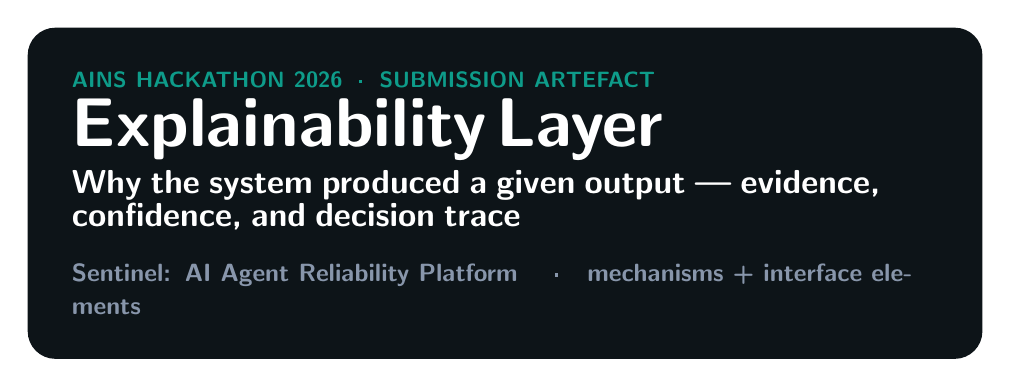
\begin{tikzpicture}
\node[rounded corners=10pt, fill=ink, inner sep=16pt, text width=\dimexpr\textwidth-32pt\relax] {%
  \color{emerald}\bfseries\footnotesize AINS HACKATHON 2026 \;\textperiodcentered\; SUBMISSION ARTEFACT \par
  \vspace{3pt}{\color{white}\fontsize{26}{30}\selectfont\bfseries Explainability Layer}\par
  \vspace{3pt}{\color{white!80}\large Why the system produced a given output --- evidence, confidence, and decision trace}\par
  \vspace{8pt}{\color{muted}\small Sentinel: AI Agent Reliability Platform \quad\textperiodcentered\quad mechanisms + interface elements}
};
\end{tikzpicture}

\vspace{6pt}
\begin{keybox}
For every output, a non-AI engineer can answer four questions without reading code:
\textbf{(1) what evidence} did the agent use, \textbf{(2) how confident} is it and where is it
uncertain, \textbf{(3) what exact sequence of steps} led here, and \textbf{(4) which step is to
blame} when something failed --- plus the ability to \textbf{re-run the exact trajectory} to
verify any of it.
\end{keybox}

\textit{\small Brief \S1.5.2: ``a mechanism or interface element showing why the system produced
a specific output, including evidence, confidence, and decision trace where applicable.'' Brief
\S1.3.4 / judging \S5 (15\%): outputs are traceable, the system communicates uncertainty, and a
non-specialist can understand why and what to do.}

% =====================================================================
\section{Five pillars of explainability}
Explainability in Sentinel is not a panel bolted on at the end --- it is a property of the
data structures themselves. Every shared object in \texttt{trace\_core} carries its own
justification, so explanation is produced \emph{by construction}.

\begin{center}
\begin{tabular}{@{}>{\bfseries}p{3.0cm} p{6.4cm} p{5.0cm}@{}}
\toprule
\rowcolor{headerbg}\multicolumn{1}{@{}>{\bfseries\color{white}}l}{Pillar} & \color{white}\bfseries Mechanism (data structure) & \color{white}\bfseries Where you see it \\
Evidence & \fld{SearchResult.attribution} (dims, terms, confidence\_margin); RCA \fld{evidence[]} cites ids & \texttt{AttributionBox}, RCA comment in Jira \\
Confidence & \fld{confidence\_score}, \fld{judge\_confidence}, per-dimension \fld{confidence} & \texttt{VerdictCard}, \texttt{ConfidenceBar} \\
Decision trace & ordered \fld{TraceRecord[]} (embedding\,$\to$\,search\,$\to$\,search\,$\to$\,chat) & \texttt{StepTimeline}, Langfuse \\
Attribution & \fld{FailureAttribution}(step, component, description, confidence) & \texttt{AttributionBox}, recommended action \\
Audit \& replay & hash-chained \fld{AuditBlock}; deterministic \fld{replay\_link} & replay screen, audit chain in D1 \\
\bottomrule
\end{tabular}
\end{center}

% =====================================================================
\section{Anatomy of an output --- the EvalVerdict}
The product of evaluation is a single structured, human-readable \texttt{EvalVerdict}. Every
field exists to be \emph{acted on}, not just read:

\begin{artifact}{EvalVerdict --- run AO-11 (trial 0)}
\fld{verdict}: \textbf{uncertain} \hfill \fld{trial\_number}: 0\\[2pt]
\fld{dimensions}: correctness 0.90 \dt\ efficiency 0.64 \dt\ safety 0.92 \dt\ reasoning\_quality 0.78\\[2pt]
\fld{failure\_attribution}: \{ step 1, component \textbf{retrieval}, ``two judge passes disagreed
on this case'', confidence 0.70 \}\\[2pt]
\fld{self\_evaluation}: \{ judge\_confidence 0.66, self\_critique ``rubric order changed the
verdict; needs review'', \textbf{flag\_for\_human true} \}\\[2pt]
\fld{recommended\_action}: ``Judge verdict is order-sensitive (position bias); human review
required.''\\[2pt]
\fld{replay\_link}: \texttt{dashboard.ahmedxsaad.me/replay/<run\_id>}
\end{artifact}

\begin{notebox}{cblue}
\textbf{Read it in one breath:} the run is \emph{uncertain}, the weak dimension is
\emph{efficiency} (0.64), the judge is not confident (0.66) so it was \emph{flagged for a
human}, and the recommended action tells the engineer exactly what to do next --- with a link to
re-run it. No AI expertise required.
\end{notebox}

% =====================================================================
\section{Pillar 1 --- Evidence (what it used)}
Retrieval is never a black box. \texttt{xqdrant} returns, for every hit, an
\texttt{Attribution} block: per-dimension and per-term contributions to the cosine score, and a
\fld{confidence\_margin} --- the gap to the next-best hit. A small margin means an ambiguous
match, which is itself a signal surfaced to the user.

\begin{artifact}{SearchResult (incidents) --- top hit for AO-11}
\fld{id}: AO-11-src \hfill \fld{score}: 0.99\\[2pt]
\fld{text}: ``Connection pool exhaustion cascading to all services''\\[2pt]
\fld{attribution.confidence\_margin}: 0.27 \;\;(strong, unambiguous match)\\[2pt]
\fld{attribution.terms}: \{ ``connection pool'': 0.41, ``cascading'': 0.22, ``exhaustion'': 0.19 \}
\end{artifact}

The drafted \texttt{RcaDraft} then \emph{cites} this evidence by id in its \fld{evidence[]}
list and records \fld{knowledge\_gaps[]} when no runbook clears the relevance floor --- so the
final Jira comment shows not just a conclusion but the grounding behind it.

% =====================================================================
\section{Pillar 2 --- Confidence and uncertainty}
The system communicates uncertainty at three nested levels, and \emph{degrades gracefully}
rather than acting when unsure:

\begin{itemize}[leftmargin=1.3em,itemsep=2pt]
  \item \textbf{Generation} --- \fld{RcaDraft.confidence\_score}; below
        \texttt{CONFIDENCE\_THRESHOLD = 0.70} the run is flagged for a human instead of
        auto-acting. Duplicate auto-linking uses a stricter \texttt{0.85} gate.
  \item \textbf{Per-dimension} --- each \fld{DimensionScore} carries its own \fld{confidence}
        alongside its score and a free-text \fld{reason}.
  \item \textbf{Verdict} --- \fld{SelfEvaluation.judge\_confidence} plus a \fld{self\_critique}.
        When the calibrated judge is order-sensitive, the verdict becomes \texttt{uncertain}
        (not a coin-flip) and \fld{flag\_for\_human} is set.
\end{itemize}

\begin{notebox}{camber}
\textbf{Self-evaluation (bonus, brief \S5).} The judge evaluates its own verdict and surfaces
low-confidence results to a human reviewer --- the system knows, and says, when it does not know.
\end{notebox}

% =====================================================================
\section{Pillar 3 --- Decision trace (the exact sequence)}
Every run is a non-lossy, ordered list of \texttt{TraceRecord} steps captured at the network
boundary by the UC2 flight recorder --- nothing is reconstructed after the fact. For AO-11:

\begin{center}
\begin{tabular}{@{}c >{\bfseries}p{2.7cm} p{4.0cm} p{5.4cm}@{}}
\toprule
\rowcolor{headerbg}\multicolumn{1}{@{}>{\color{white}\bfseries}c}{\#} & \color{white}\bfseries Step & \color{white}\bfseries Model / tool & \color{white}\bfseries Readable preview \\
0 & embedding & bge-base-en-v1.5 & ``embed 1 text \dots'' $\to$ 768-dim vector \\
1 & vector search & xqdrant incidents & top hit 0.99 (connection-pool exhaustion) \\
2 & vector search & xqdrant runbooks & ``DB connection pool exhaustion'' 0.72 \\
3 & chat (RCA) & llama-3.1-8b & hypothesis + cited evidence + severity \\
\bottomrule
\end{tabular}
\end{center}

Each step stores a human-readable input/output preview (not raw JSON), the model id, and the
operation, so the dashboard \texttt{StepTimeline} reads as a story. The same calls are exported
to \textbf{Langfuse} as GenAI traces for an engineer who wants the raw prompt/response/latency.

% =====================================================================
\section{Pillar 4 --- Failure attribution (who is to blame)}
A failing run is mapped onto a small DAG, \texttt{retrieval} $\to$ \texttt{planning} $\to$
\texttt{execution}, and the first step showing a failure signal is blamed --- with a confidence
graded by how explicit the signal is:

\begin{center}
\begin{tabular}{@{}p{6.8cm} c p{5.2cm}@{}}
\toprule
\rowcolor{headerbg}\multicolumn{1}{@{}>{\bfseries\color{white}}l}{Signal} & \color{white}\bfseries Confidence & \color{white}\bfseries Component \\
explicit error / \texttt{success=false} & 0.90 & as classified \\
retrieval returned no results & 0.70 & retrieval \\
execution produced no key/id outcome & 0.70 & execution \\
no explicit signal (blame last step) & 0.50 & fallback \\
\bottomrule
\end{tabular}
\end{center}
The output is a sentence, not a stack trace: \emph{``Step 2, retrieval, returned no results
(confidence 0.7)''} --- the difference between ``it failed'' and ``open replay and fix the
retrieval step.''

% =====================================================================
\section{Pillar 5 --- Audit and deterministic replay}
Explainability is only trustworthy if the record cannot be quietly altered and the claim can be
reproduced. Two mechanisms guarantee this:

\begin{itemize}[leftmargin=1.3em,itemsep=2pt]
  \item \textbf{Tamper-evident audit} --- every step is an \texttt{AuditBlock} with a
        \fld{payload\_hash} (SHA-256 of canonical JSON), an \fld{hmac} (signed with a server
        key), and a \fld{prev\_hash} linking it to the previous step. Written \emph{write-ahead}
        (before execution), the chain proves the trajectory was not edited after the fact.
  \item \textbf{Deterministic replay} --- \texttt{replay\_link} re-runs the exact trajectory
        from the cassette with \textbf{zero live calls}; a request the agent never originally
        made shows up as a \emph{divergence}. \texttt{bisect} finds the first diverging step
        between two runs, and mid-replay \texttt{inject} lets an engineer change one response and
        watch the path change --- explaining \emph{counterfactually} why a step mattered.
\end{itemize}

% =====================================================================
\section{Interface elements --- where to look}
The mechanisms above surface in the dashboard (\texttt{dashboard.ahmedxsaad.me}). A reviewer
never needs the code:

\begin{center}
\begin{tabular}{@{}p{5.4cm} p{4.0cm} p{5.4cm}@{}}
\toprule
\rowcolor{headerbg}\multicolumn{1}{@{}>{\bfseries\color{white}}l}{Question} & \color{white}\bfseries Screen & \color{white}\bfseries Interface element \\
What did the agent do? & \texttt{/runs/<id>} & \texttt{StepTimeline} (operation-aware) \\
Did it do it right? & \texttt{/verdicts/<id>} & \texttt{VerdictCard} + \texttt{DimensionTable} \\
Why this verdict? & \texttt{/verdicts/<id>} & \texttt{AttributionBox} + self-critique \\
Can you prove it? & \texttt{/replay/<id>} & replay (0 live calls) + bisect + inject \\
How reliable overall? & \texttt{/} \& \texttt{/reliability} & \texttt{ReliabilityRing}, drift, $\kappa$ \\
Raw LLM calls? & Langfuse & per-call prompt / response / latency \\
\bottomrule
\end{tabular}
\end{center}

% =====================================================================
\section{Worked example --- AO-11 end to end}
\begin{notebox}{cteal}
\textbf{1. Evidence} --- incident embedded once; xqdrant returns ``connection-pool exhaustion''
at 0.99 (margin 0.27) and a DB-pool runbook at 0.72. \textbf{2. Decision trace} --- four taped
steps (embed $\to$ search $\to$ search $\to$ RCA), each replayable. \textbf{3. Confidence} ---
the RCA cites those ids; the two calibrated judge passes disagree, so judge\_confidence drops and
the verdict is \texttt{uncertain}. \textbf{4. Attribution} --- the unstable step + component are
named; \textbf{5. Audit/replay} --- the run replays with 0 live calls and an \texttt{AO} Jira
Incident is auto-filed for the human. Every claim above is a field a reviewer can open and check.
\end{notebox}

\begin{keybox}
\textbf{Bottom line.} Explanation is structural, not cosmetic: evidence with attribution,
three levels of confidence, a non-lossy decision trace, per-step blame, and a tamper-evident,
re-runnable record --- each surfaced as a concrete interface element a non-specialist can act on.
\end{keybox}

\end{document}
